\documentclass{article}
\usepackage{graphicx}
\usepackage[utf8]{inputenc}

\title{Latex PPNM exercise}
\author{Esben Porat}
\date{May 2022}

\begin{document}

\maketitle

\section{The Exponential Function}
The exponential function, along with the natural logarithmic function, were two important functions for performing calculations before modern calculators were invented. Their functionality are similar in the sense that $\ln(x\cdot2) = \ln(x) + \ln(2)$ and $\exp(x\cdot2) = \exp(x) \cdot\exp(2)$ can be used to compress calculations in ways multiplication by hand cannot do, and look-up tables of the values of these functions could then be used to approximate calculations that were otherwise orders of magnitude larger than what was otherwise feasible.\\

The exponential function itself also has a variety of interesting properties in the realm of calculus. Its derivative is by definition itself, from which we can easily find a power series representation of the function:
$$\sum_{n=0}^{\infty} \frac{x^n}{n!}$$
The tail of this infinite series is absolutely convergent by the virtue of the factorial eventually outpacing the exponential.\\
We can do a few interesting things using this definition of the exponential - among them, easily find the Euler formula:
$$\exp(ix) = \cos(x) + i\sin(x)$$
Here, the absolute convergence of the exponential power series lets us rearrange the terms to group them as real and imaginary components, and the sums for each of these are equivalent to the Taylor expansions at $x=0$ for the cosine and sine functions.

\section{The Implementation}
The given implementation truncates the power series at $n=10$, and as a result is met with some challenges: If x is large enough that the value of each term in the series is still increasing by the tenth term, the truncation is a bad approximation. To solve this, the implementation makes use of 2 things; the fact that for $x < 1$, the size of each successive term will always be smaller than the preceding one, and the fact that $\exp(x / 2)^2 = \exp(x)$. By only allowing $|x|\leq \frac{1}{8}$, we ensure that the implementation is a good approximation to the full sum.\\

In addition to this, the implementation also rewrites the sum in a way which minimizes computational load. Exponentials are slow to calculate; $x^{10}$ requires 9 multiplications, and factorials are just as bad, with $10!$ also requiring 9 multiplications. This means that each successive term $n$ requires $2\cdot n!$ operations. The rewritten sum 'reuses' previous factorials and exponentials when calculating the succeeding term, and as such only requires 3 operations per term added: One multiplication by a factor that is calculated by one addition of a value calculated by one division.\\

In the figure below is an example of the implementation plotted against the System.Math.Exp value of $x$-values between -2 and 2:

\begin{figure}[h!]
    \centering
    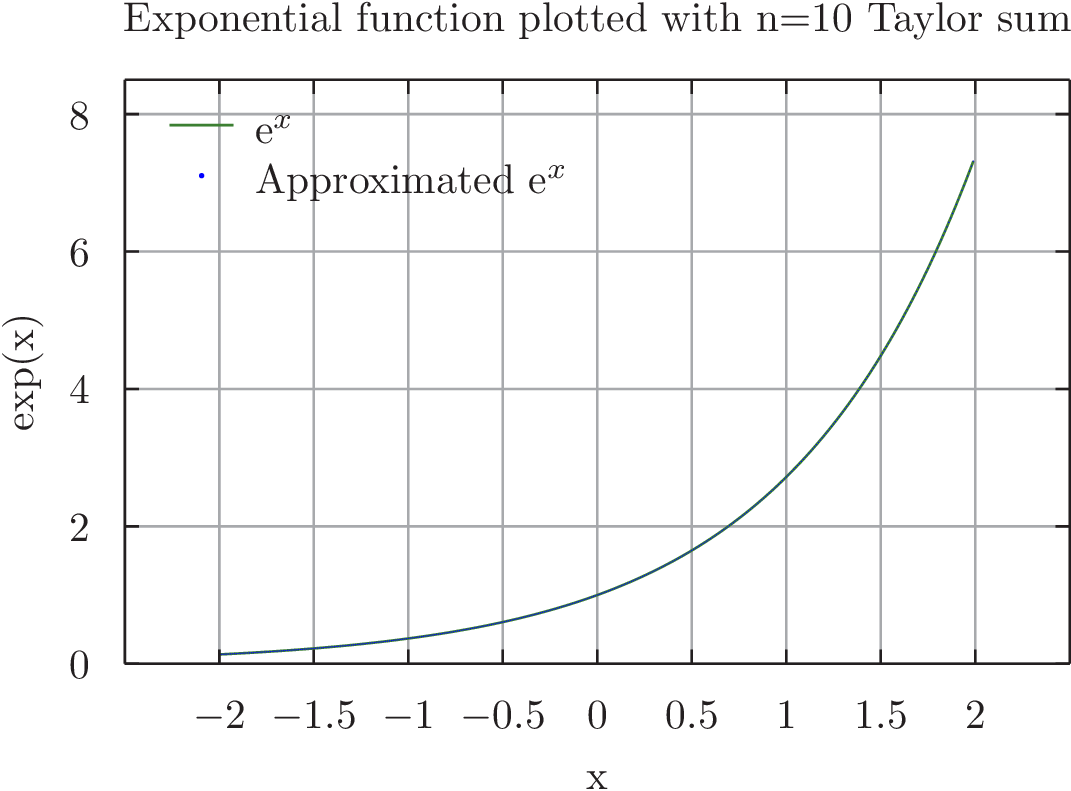
\includegraphics[width=\linewidth]{exp.pyxplot.png}
    \caption{The two functions are all but indistinguishable.}
    \label{}
\end{figure}

\end{document}
